\documentclass{standalone}
\usepackage{tikz}
\usetikzlibrary{patterns, positioning}
\usepackage[sfdefault]{ClearSans} %% option 'sfdefault' activates Clear Sans as the default text font
\usepackage[T1]{fontenc}

\begin{document}
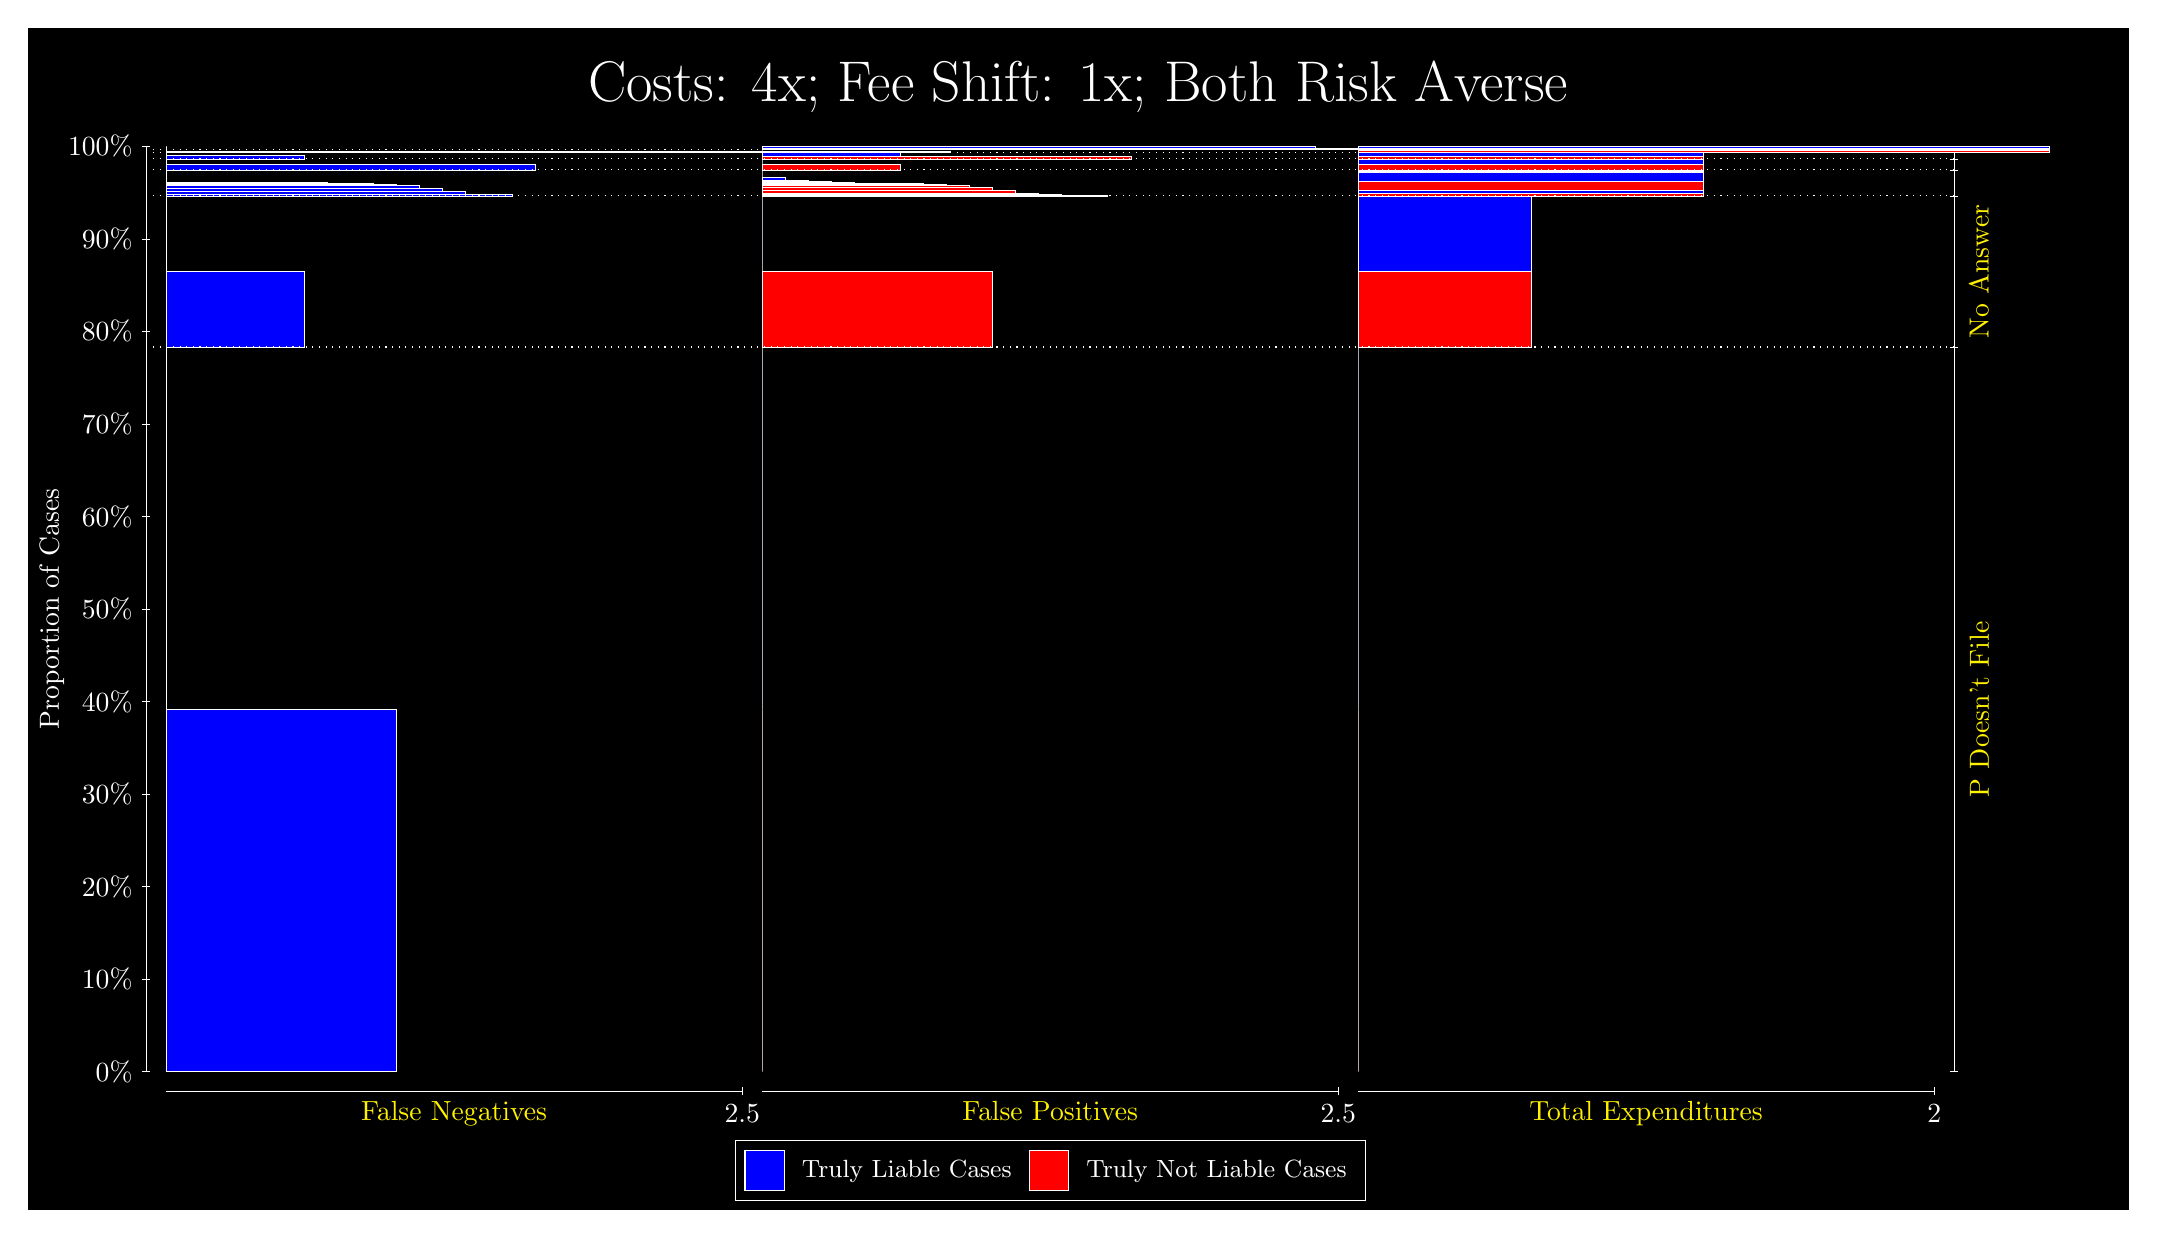
\begin{tikzpicture}
\draw[fill=black] (0,0) rectangle (26.667,15);
\draw[text=white] (0,13.5) rectangle (26.667,15) node[midway] {\huge Costs: 4x; Fee Shift: 1x; Both Risk Averse};
\draw[white, very thin] (1.5,1.75) -- (1.5,13.5);
\node[rotate=90, text=white, anchor=center] at (0.3, 7.625) {Proportion of Cases};
\draw[white, very thin] (1.45,1.75) -- (1.55,1.75);
\node[text=white, anchor=east] at (1.45, 1.75) {0\%};
\draw[white, very thin] (1.45,2.925) -- (1.55,2.925);
\node[text=white, anchor=east] at (1.45, 2.925) {10\%};
\draw[white, very thin] (1.45,4.1) -- (1.55,4.1);
\node[text=white, anchor=east] at (1.45, 4.1) {20\%};
\draw[white, very thin] (1.45,5.275) -- (1.55,5.275);
\node[text=white, anchor=east] at (1.45, 5.275) {30\%};
\draw[white, very thin] (1.45,6.45) -- (1.55,6.45);
\node[text=white, anchor=east] at (1.45, 6.45) {40\%};
\draw[white, very thin] (1.45,7.625) -- (1.55,7.625);
\node[text=white, anchor=east] at (1.45, 7.625) {50\%};
\draw[white, very thin] (1.45,8.8) -- (1.55,8.8);
\node[text=white, anchor=east] at (1.45, 8.8) {60\%};
\draw[white, very thin] (1.45,9.975) -- (1.55,9.975);
\node[text=white, anchor=east] at (1.45, 9.975) {70\%};
\draw[white, very thin] (1.45,11.15) -- (1.55,11.15);
\node[text=white, anchor=east] at (1.45, 11.15) {80\%};
\draw[white, very thin] (1.45,12.325) -- (1.55,12.325);
\node[text=white, anchor=east] at (1.45, 12.325) {90\%};
\draw[white, very thin] (1.45,13.5) -- (1.55,13.5);
\node[text=white, anchor=east] at (1.45, 13.5) {100\%};

\draw[white, very thin] (24.457,1.75) -- (24.457,13.5);
\draw[white, very thin] (24.407,1.75) -- (24.507,1.75);
\node[anchor=west] at (24.407, 1.75) {};
\draw[white, very thin] (24.407,10.951) -- (24.507,10.951);
\node[anchor=west] at (24.407, 10.951) {};
\draw[white, very thin] (24.407,12.87) -- (24.507,12.87);
\node[anchor=west] at (24.407, 12.87) {};
\draw[white, very thin] (24.407,13.201) -- (24.507,13.201);
\node[anchor=west] at (24.407, 13.201) {};
\draw[white, very thin] (24.407,13.34) -- (24.507,13.34);
\node[anchor=west] at (24.407, 13.34) {};
\draw[white, very thin] (24.407,13.422) -- (24.507,13.422);
\node[anchor=west] at (24.407, 13.422) {};
\draw[white, very thin] (24.407,13.462) -- (24.507,13.462);
\node[anchor=west] at (24.407, 13.462) {};
\draw[white, very thin] (24.407,13.5) -- (24.507,13.5);
\node[anchor=west] at (24.407, 13.5) {};

\draw[white, very thin, fill=blue] (1.75,1.75) rectangle (4.6775,6.3507);
\draw[white, very thin, fill=red] (1.75,6.3507) rectangle (1.75,10.951);
\draw[white, very thin, fill=blue] (1.75,10.951) rectangle (3.5065,11.909);
\draw[white, very thin, fill=red] (1.75,11.909) rectangle (1.75,12.87);
\draw[white, very thin, fill=blue] (1.75,12.87) rectangle (6.1413,12.885);
\draw[white, very thin, fill=blue] (1.75,12.885) rectangle (5.8486,12.893);
\draw[white, very thin, fill=blue] (1.75,12.893) rectangle (5.5558,12.927);
\draw[white, very thin, fill=blue] (1.75,12.927) rectangle (5.2631,12.966);
\draw[white, very thin, fill=blue] (1.75,12.966) rectangle (4.9703,13.004);
\draw[white, very thin, fill=blue] (1.75,13.004) rectangle (4.6775,13.019);
\draw[white, very thin, fill=blue] (1.75,13.019) rectangle (4.3848,13.03);
\draw[white, very thin, fill=blue] (1.75,13.03) rectangle (4.092,13.035);
\draw[white, very thin, fill=blue] (1.75,13.035) rectangle (3.7993,13.04);
\draw[white, very thin, fill=red] (1.75,13.04) rectangle (1.75,13.201);
\draw[white, very thin, fill=blue] (1.75,13.201) rectangle (6.4341,13.269);
\draw[white, very thin, fill=red] (1.75,13.269) rectangle (1.75,13.34);
\draw[white, very thin, fill=blue] (1.75,13.34) rectangle (3.5065,13.383);
\draw[white, very thin, fill=red] (1.75,13.383) rectangle (1.75,13.422);
\draw[white, very thin, fill=blue] (1.75,13.422) rectangle (11.704,13.435);
\draw[white, very thin, fill=red] (1.75,13.435) rectangle (1.75,13.462);
\draw[white, very thin, fill=red] (1.75,13.462) rectangle (1.75,13.476);
\draw[white, very thin, fill=blue] (1.75,13.476) rectangle (1.75,13.5);
\draw[white, very thin, fill=red] (9.3189,1.75) rectangle (9.3189,6.3507);
\draw[white, very thin, fill=blue] (9.3189,6.3507) rectangle (9.3189,10.951);
\draw[white, very thin, fill=red] (9.3189,10.951) rectangle (12.246,11.913);
\draw[white, very thin, fill=blue] (9.3189,11.913) rectangle (9.3189,12.87);
\draw[white, very thin, fill=red] (9.3189,12.87) rectangle (13.71,12.875);
\draw[white, very thin, fill=red] (9.3189,12.875) rectangle (13.417,12.88);
\draw[white, very thin, fill=red] (9.3189,12.88) rectangle (13.125,12.891);
\draw[white, very thin, fill=red] (9.3189,12.891) rectangle (12.832,12.905);
\draw[white, very thin, fill=red] (9.3189,12.905) rectangle (12.539,12.94);
\draw[white, very thin, fill=red] (9.3189,12.94) rectangle (12.246,12.976);
\draw[white, very thin, fill=red] (9.3189,12.976) rectangle (11.954,13.008);
\draw[white, very thin, fill=red] (9.3189,13.008) rectangle (11.661,13.016);
\draw[white, very thin, fill=red] (9.3189,13.016) rectangle (11.368,13.032);
\draw[white, very thin, fill=blue] (9.3189,13.032) rectangle (10.783,13.037);
\draw[white, very thin, fill=blue] (9.3189,13.037) rectangle (10.49,13.042);
\draw[white, very thin, fill=blue] (9.3189,13.042) rectangle (10.197,13.053);
\draw[white, very thin, fill=blue] (9.3189,13.053) rectangle (9.9044,13.067);
\draw[white, very thin, fill=blue] (9.3189,13.067) rectangle (9.6116,13.106);
\draw[white, very thin, fill=blue] (9.3189,13.106) rectangle (9.3189,13.201);
\draw[white, very thin, fill=red] (9.3189,13.201) rectangle (11.075,13.273);
\draw[white, very thin, fill=blue] (9.3189,13.273) rectangle (9.3189,13.34);
\draw[white, very thin, fill=red] (9.3189,13.34) rectangle (14.003,13.379);
\draw[white, very thin, fill=blue] (9.3189,13.379) rectangle (11.075,13.422);
\draw[white, very thin, fill=red] (9.3189,13.422) rectangle (9.3189,13.448);
\draw[white, very thin, fill=blue] (9.3189,13.448) rectangle (9.3189,13.462);
\draw[white, very thin, fill=red] (9.3189,13.462) rectangle (19.273,13.476);
\draw[white, very thin, fill=blue] (9.3189,13.476) rectangle (16.345,13.5);
\draw[white, very thin, fill=red] (16.888,1.75) rectangle (16.888,6.3507);
\draw[white, very thin, fill=blue] (16.888,6.3507) rectangle (16.888,10.951);
\draw[white, very thin, fill=red] (16.888,10.951) rectangle (19.083,11.913);
\draw[white, very thin, fill=blue] (16.888,11.913) rectangle (19.083,12.87);
\draw[white, very thin, fill=red] (16.888,12.87) rectangle (21.279,12.906);
\draw[white, very thin, fill=blue] (16.888,12.906) rectangle (21.279,12.944);
\draw[white, very thin, fill=red] (16.888,12.944) rectangle (21.279,13.054);
\draw[white, very thin, fill=blue] (16.888,13.054) rectangle (21.279,13.17);
\draw[white, very thin, fill=red] (16.888,13.17) rectangle (21.279,13.185);
\draw[white, very thin, fill=blue] (16.888,13.185) rectangle (21.279,13.201);
\draw[white, very thin, fill=red] (16.888,13.201) rectangle (21.279,13.273);
\draw[white, very thin, fill=blue] (16.888,13.273) rectangle (21.279,13.34);
\draw[white, very thin, fill=red] (16.888,13.34) rectangle (21.279,13.379);
\draw[white, very thin, fill=blue] (16.888,13.379) rectangle (21.279,13.422);
\draw[white, very thin, fill=red] (16.888,13.422) rectangle (25.67,13.448);
\draw[white, very thin, fill=blue] (16.888,13.448) rectangle (25.67,13.462);
\draw[white, very thin, fill=red] (16.888,13.462) rectangle (25.67,13.476);
\draw[white, very thin, fill=blue] (16.888,13.476) rectangle (25.67,13.5);
\draw[white, dotted] (1.5,10.951) -- (24.457,10.951);
\draw[white, dotted] (1.5,12.87) -- (24.457,12.87);
\draw[white, dotted] (1.5,13.201) -- (24.457,13.201);
\draw[white, dotted] (1.5,13.34) -- (24.457,13.34);
\draw[white, dotted] (1.5,13.422) -- (24.457,13.422);
\draw[white, dotted] (1.5,13.462) -- (24.457,13.462);
\draw[white, very thin] (1.75,1.5) -- (9.0689,1.5);
\node[text=yellow, anchor=north] at (5.4094, 1.5) {False Negatives};
\draw[white, very thin] (9.0689,1.45) -- (9.0689,1.55);
\node[text=white, anchor=north] at (9.0689, 1.45) {2.5};

\draw[white, very thin] (9.3189,1.5) -- (16.638,1.5);
\node[text=yellow, anchor=north] at (12.978, 1.5) {False Positives};
\draw[white, very thin] (16.638,1.45) -- (16.638,1.55);
\node[text=white, anchor=north] at (16.638, 1.45) {2.5};

\draw[white, very thin] (16.888,1.5) -- (24.207,1.5);
\node[text=yellow, anchor=north] at (20.547, 1.5) {Total Expenditures};
\draw[white, very thin] (24.207,1.45) -- (24.207,1.55);
\node[text=white, anchor=north] at (24.207, 1.45) {2};

\node[text=yellow, centered, rotate=90] at (24.777, 6.3507) {P Doesn't File};
\node[text=yellow, centered, rotate=90] at (24.777, 11.911) {No Answer};






\draw (12.978300999999998,1.5) node[draw=none] (baseCoordinate) {};
\begin{scope}[align=center]
        \matrix[scale=0.5, draw=white, below=0.5cm of baseCoordinate, nodes={draw}, column sep=0.1cm]{
            \node[rectangle, draw, minimum width=0.5cm, minimum height=0.5cm, fill=blue] {}; &
            \node[draw=none, font=\small, text=white] (B) {Truly Liable Cases}; &
            \node[rectangle, draw, minimum width=0.5cm, minimum height=0.5cm, fill=red] {}; &
            \node[draw=none, font=\small, text=white] (B) {Truly Not Liable Cases}; \\
            };
\end{scope}

\end{tikzpicture}
\end{document}